\documentclass{standalone}
\usepackage{tikz}

\begin{document}
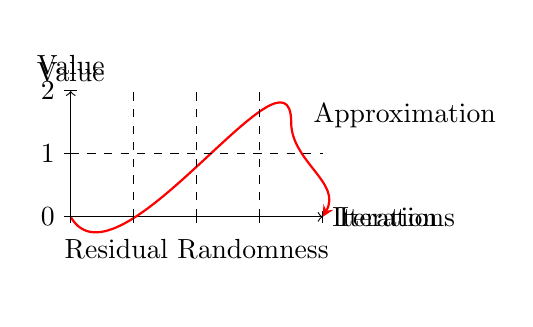
\begin{tikzpicture}[scale=0.8]
    % Define coordinates
    \coordinate (origin) at (0,0);
    \coordinate (x1) at (4,0);
    \coordinate (y1) at (0,2);

    % Draw axes
    \draw[->] (origin) -- (x1) node[right] {Iteration};
    \draw[->] (origin) -- (y1) node[above] {Value};

    % Plot the line
    \draw[-stealth, thick, red] (0,0) to[out=-60,in=90] (3.5,1.5) to[out=-90,in=60] (4,0);

    % Add labels
    \node at (2,-0.2) [below] {Residual Randomness};
    \node at (3.7,1.6) [right] {Approximation};

    % Add grid
    \draw[dashed] (0,1) -- (4,1);
    \draw[dashed] (1,0) -- (1,2);
    \draw[dashed] (2,0) -- (2,2);
    \draw[dashed] (3,0) -- (3,2);

    % Add tick marks
    \foreach \x in {0,1,2,3,4} {
        \draw (\x,-0.1) -- (\x,0.1);
    }
    \foreach \y in {0,1,2} {
        \draw (-0.1,\y) -- (0.1,\y);
    }

    % Add axis labels
    \node at (-0.1,0) [left] {0};
    \node at (-0.1,1) [left] {1};
    \node at (-0.1,2) [left] {2};
    \node at (4.1,0) [right] {Iterations};
    \node at (0,2.1) [above] {Value};
\end{tikzpicture}
\end{document}